\documentclass{beamer}

\usepackage[utf8]{inputenc}
\usepackage{graphicx} 


%Information to be included in the title page:
\title{Laboratorio 3}
\author{Alvaro Frias Garay - Ary Lautaro Di Bartolo}
\institute{Universidad Nacional de Córdoba - Universidad Nacional de Cuyo}
\date{2021}

\begin{document}
    \frame{\titlepage}

    \begin{frame}
        \frametitle{Estrategias e Implementaciones}
        \begin{itemize}
            \item Paralelizar tinymc no vectorizado
            \item Paralelizar tinymc vectorizado
        \end{itemize}
    \end{frame}

    \begin{frame}
        \frametitle{Paralelizando el tinymc no vectorizado}

        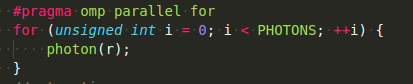
\includegraphics[width=2in]{imagenes/opt_omp_lin_1.png} \pause
        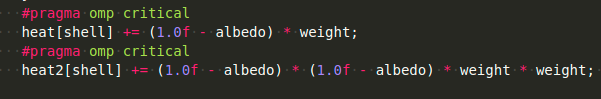
\includegraphics[width=2in]{imagenes/opt_omp_lin_2.png}
    \end{frame}

    \begin{frame}
        \frametitle{Paralelizando el tinymc no vectorizado}
        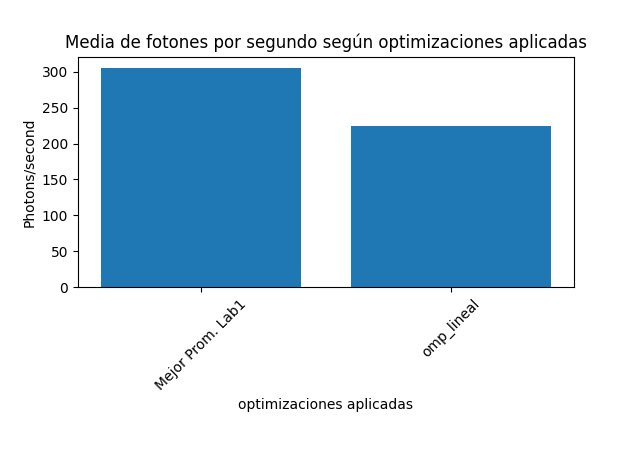
\includegraphics[width=4in]{imagenes/comp_prom_1.png}
    \end{frame}

    \begin{frame}
        \frametitle{Paralelizando el tinymc no vectorizado}
        Principales Problemas
        \begin{itemize}
            \item False sharing
            \item scheduling no dinámico
        \end{itemize}
    \end{frame}

    \begin{frame}
        \frametitle{Paralelizando el tinymc no vectorizado}
        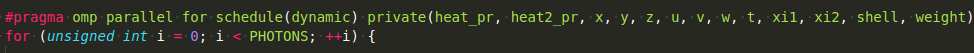
\includegraphics[width=4in]{imagenes/opt_omp_lin_3.png}

    \end{frame}

    \begin{frame}
        \frametitle{Paralelizando el tinymc no vectorizado}

        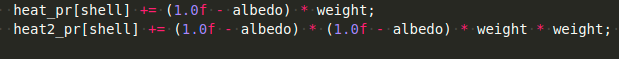
\includegraphics[width=3in]{imagenes/opt_omp_lin_4.png} \pause
        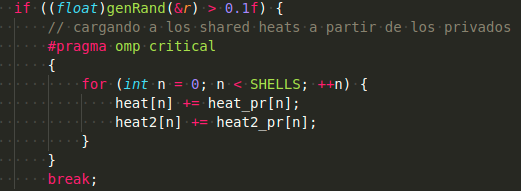
\includegraphics[width=2in]{imagenes/opt_omp_lin_5.png}

    \end{frame}

    \begin{frame}
        \frametitle{Paralelizando el tinymc no vectorizado}
        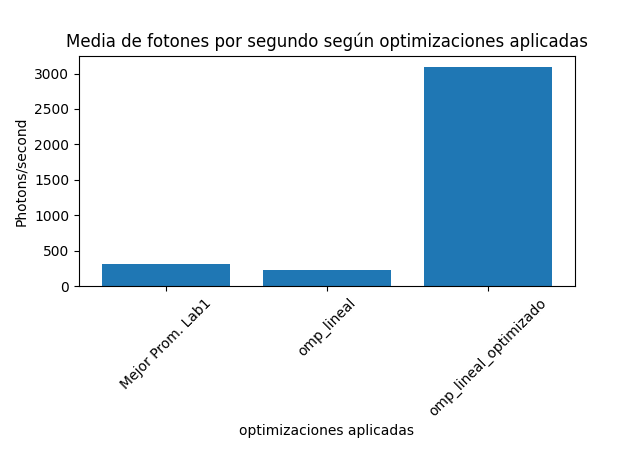
\includegraphics[width=4in]{imagenes/comp_prom_2.png}
    \end{frame}

    \begin{frame}
        \frametitle{Paralelizando tinymc vectorizado}
        \begin{itemize}
            \item Muy difícil paralelizar intrinsics
            \item Refactorizar el código
        \end{itemize}
    \end{frame}

    \begin{frame}
        \frametitle{Paralelizando tinymc vectorizado}
        
\includegraphics[width=3in]{imagenes/omp_vec_1.png}

        OpenMP incluye directivas para vectorizar for loops

    \end{frame}

    \begin{frame}
        \frametitle{Detalle de vectorización con OpenMP}
         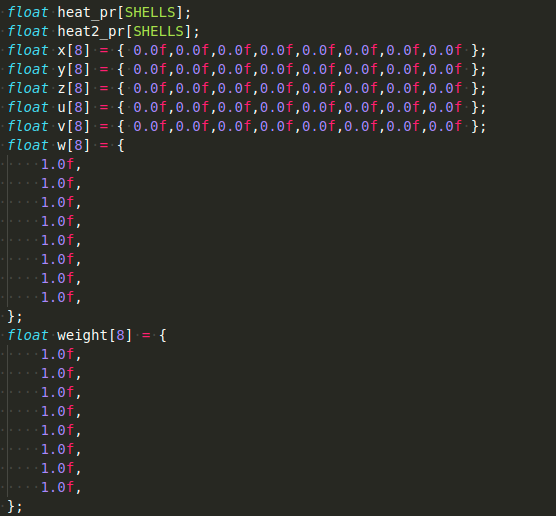
\includegraphics[width=4in, height=3in]{imagenes/omp_vec_2.png}
    \end{frame}

    \begin{frame}
        \frametitle{Detalle de vectorización con OpenMP}
        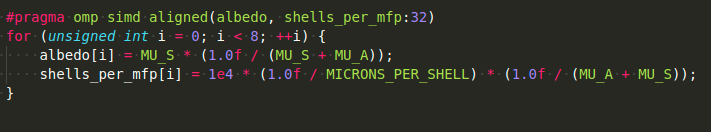
\includegraphics[width=4in]{imagenes/omp_vec_3.png}
    \end{frame}

    \begin{frame}
        \frametitle{Detalle de vectorización con OpenMP}
        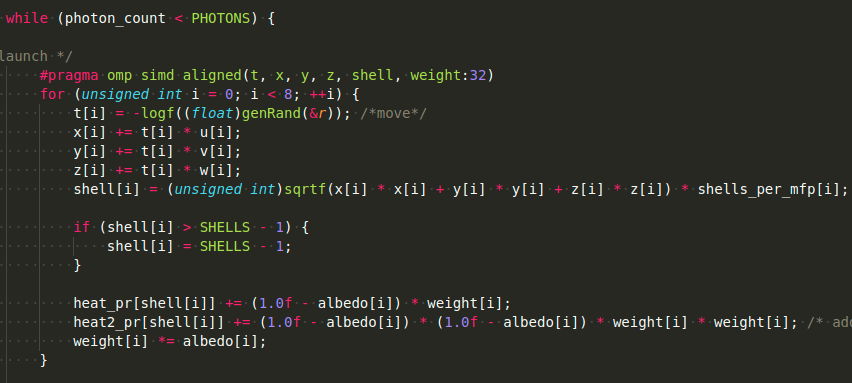
\includegraphics[width=4in]{imagenes/omp_vec_4.png}

    \end{frame}

    \begin{frame}
        \frametitle{Detalle de vectorización con OpenMP}
        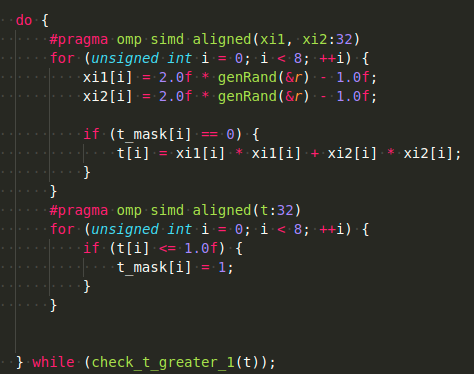
\includegraphics[width=4in]{imagenes/omp_vec_5.png}

    \end{frame}

    \begin{frame}
        \frametitle{Detalle de vectorización con OpenMP}
        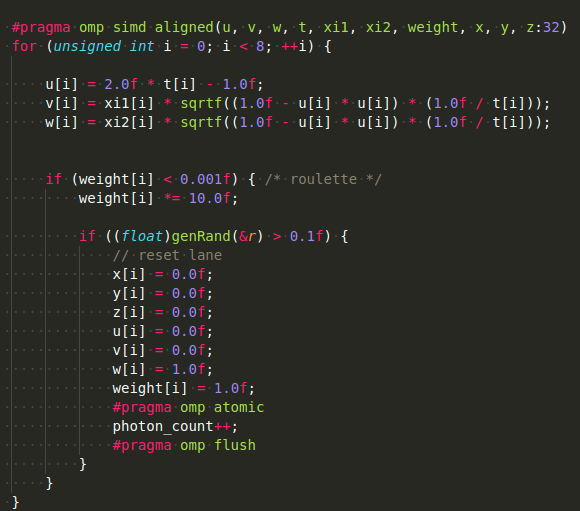
\includegraphics[width=4in, height=3in]{imagenes/omp_vec_6.png}

    \end{frame}

    \begin{frame}
        \frametitle{Detalle de vectorización con OpenMP}
        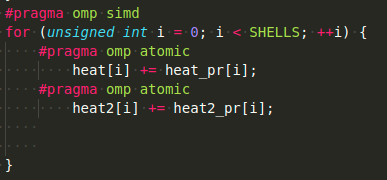
\includegraphics[width=4in]{imagenes/omp_vec_7.png}

    \end{frame}

    \begin{frame}
        \frametitle{Detalle de vectorización con OpenMP}
        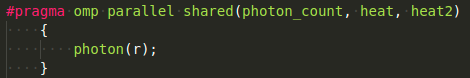
\includegraphics[width=4in]{imagenes/omp_vec_9.png}

    \end{frame}

    \begin{frame}
        \frametitle{Comparación de velocidades}
        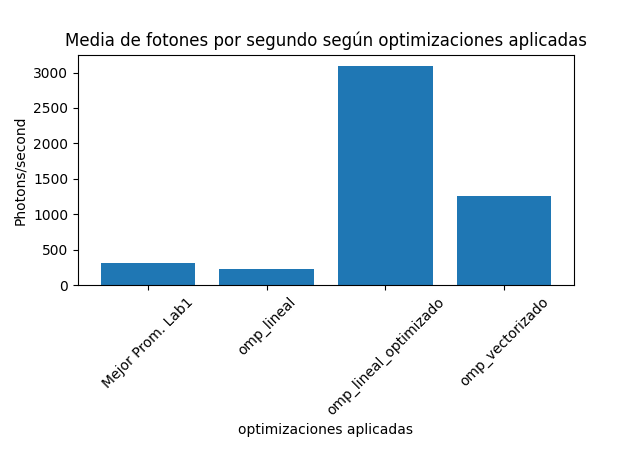
\includegraphics[width=4in]{imagenes/media_comp_3.png}
    \end{frame}

    \begin{frame}
        \frametitle{Scaling según número de threads}
        2 Threads
        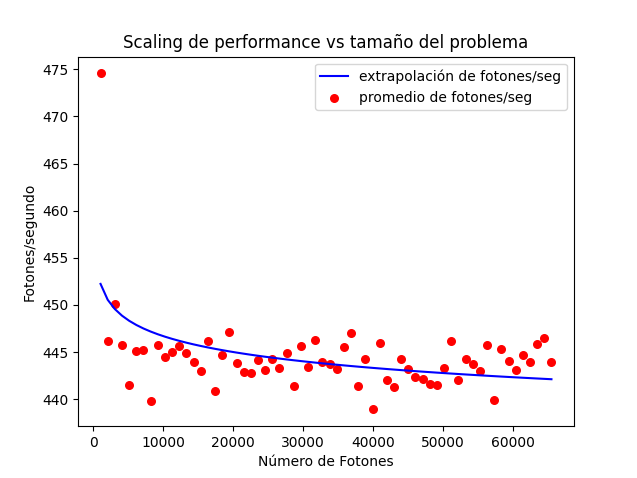
\includegraphics[width=4in]{imagenes/scaling_2threads_alv.png}
    \end{frame}

    \begin{frame}
        \frametitle{Scaling según número de threads}
        4 Threads
        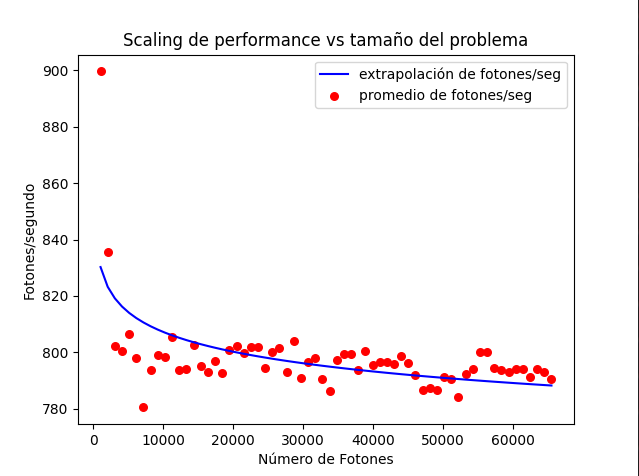
\includegraphics[width=4in]{imagenes/scaling_4threads_alv.png}
    \end{frame}

    \begin{frame}
        \frametitle{Scaling según número de threads}
        8 Threads
        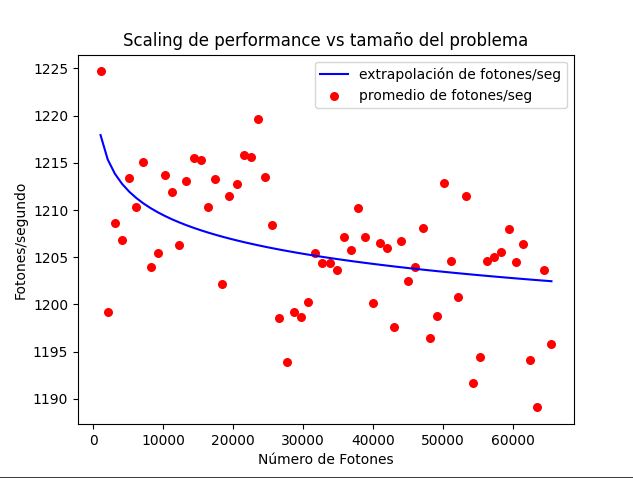
\includegraphics[width=4in]{imagenes/scaling_8threads_alv.png}
    \end{frame}

	\begin{frame}
		\frametitle{Roofline}

		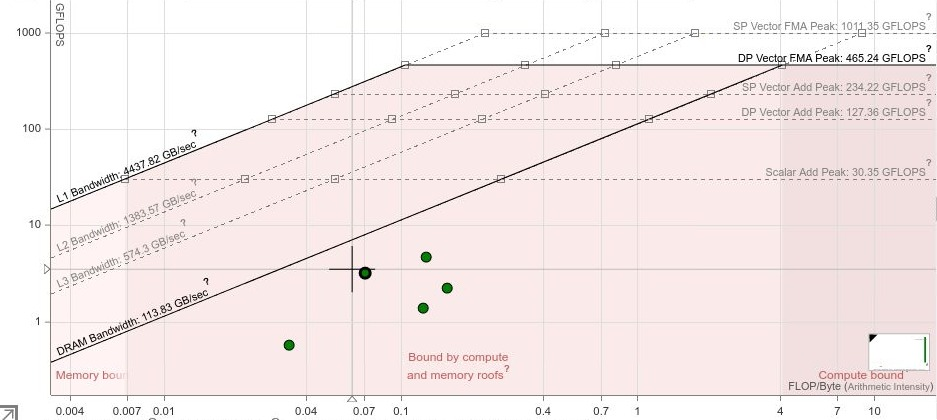
\includegraphics[width=4in]{imagenes/roofline.jpeg}
	\end{frame}

    \begin{frame}
        \frametitle{Conclusiones}
        \begin{itemize}
            \item Código mucho más legible
            \item Mejoras notables en velocidad respecto a versiones anteriores
        \end{itemize}
    \end{frame}

    \begin{frame}
        \frametitle{Potenciales Mejoras}
        \begin{itemize}
            \item Seguimos sin vectorizar el generador de números
        \end{itemize}
    \end{frame}

\end{document}